





\section{Abstract}


\tmpsection{One or two sentences providing a basic introduction to the field}
% comprehensible to a scientist in any discipline.
\lettr{I}t is still unclear what factors determine the number of pathogens a wild species carries.
But once understood, these factors could provide a way to prioritise surveillance of wild populations for zoonotic disease and make predictions as to how pathogen richness will respond to global change.


\tmpsection{Two to three sentences of more detailed background}
% comprehensible to scientists in related disciplines.

% Theory led.

The pattern of contacts between individuals (i.e. population structure) has long been known to strongly affect epidemic processes.
Theory suggests that population structure can promote pathogen richness while the ecological literature generally assumes it will decrease richness.


\tmpsection{One sentence clearly stating the general problem (the gap)}
% being addressed by this particular study.

Previous studies in wild bat populations have had contradictory results and the different measures of population structure have different shortcomings.
There is therefore a need for more robust comparative studies testing for a relationship between pathogen richness and population structure.

\tmpsection{One sentence summarising the main result}
%  (with the words “here we show” or their equivalent).

Here I used comparative data to test whether population structure influences pathogen richness using bats as a case study as they have been associated with a number of important, recent zoonotic outbreaks.
Unlike previous studies I used two measures of population structure: a novel measure, number of subspecies, and a more careful application of genetic measures which have been used previously.
I find that both of these measures are positively associated with pathogen richness and are probably in the best supported model.


\tmpsection{Two or three sentences explaining what the main result reveals in direct comparison to what was thoughts to be the case previously}
% or how the main result adds to previous knowledge

My results add more robust support to the hypothesis that pathogen structure promotes pathogen richness in bats and lends clarity to the contradictory results previously published.
The results support predictions from theory.
They contradict the assumption commonly made in the ecological literature that factors that increase $R_0$ should increase pathogen richness implying that competitive processes amongst pathogens are stronger than previously thought.


\tmpsection{One or two sentences to put the results into a more general context.}

Although my analysis implies that population structure does promote pathogen richness in bats, the weakness of the relationship and the difficulty in obtaining some measurements means this is probably not a usefully predictive factor on it's own for optimising zoonotic surveillance.
However, the relationship has implications for global change, implying that increased habitat fragmentation might promote greater viral richness in bats.





%%%%%%%%%%%%%%%%%%%%%%%%%%%%%%%%%%%%%%%%%%%%%%%%%%%%%%%%%%%%%%%%%%%%%%%%%%%%%%%%%%%%%%%%%%%%%%%%%%%%%%%%%%%%%%%%%%%%%%%%%%%%%%%%%%%%%%%%%%%%%%%%%%%%%%%%%%%

\section{Introduction}

%%%%%%%%%%%%%%%%%%%%%%%%%%%%%%%%%%%%%%%%%%%%%%%%%%%%%%%%%%%%%%%%%%%%%%%%%%%%%%%%%%%%%%%%%%%%%%%%%%%%%%%%%%%%%%%%%%%%%%%%%%%%%%%%%%%%%%%%%%%%%%%%%%%%%%%%%%%

\tmpsection{General Intro}
The number of pathogen species carried by a host species has important consequences for the ecology of the host and the probability that the host will be a reservoir of a zoonotic pathogen.
However, the factors that affect pathogen richness are poorly understood.



\tmpsection{Specific Intro}



\tmpsection{Theoretical background}

%Think this ref is right but need to check.
Single pathogen models show that increasing population structure simply slows disease spread and makes establishment less likely \cite{colizza2007invasion, vespignani2008reaction}.
In the ecological literature this is often taken as predicting that increased population structure will decrease pathogen richness \cite{nunn2003comparative, morand2000wormy}.
However, models of competition between multiple pathogens show that in unstructured populations a competitive exclusion process occurs but that splitting the population into two patches allows coexistence \cite{qiu2013vector,allen2004sis, nunes2006localized}.


\tmpsection{Previous Studies}

Three studies have used comparative data to test for an association between population structure and viral richness.
A study on 15 African bats found a positive relationship between distribution fragmentation and viral richness \cite{maganga2014bat} while a study on 20 South-East Asian bats found the opposite relationship \cite{gay2014parasite}. 
A global study on 33 bats found a positive relationship between $F_{ST}$ --- a measure of genetic structure --- and viral richness \cite{turmelle2009correlates}. 
However, this study included measures using mtDNA which only measures female dispersal which may have biased the results many bat species show female philopatry \cite{kerth2002extreme, hulva2010mechanisms}.
Furthermore, this study used measures of $F_{ST}$ irrespective of the study scale with studies covering from tens \cite{mccracken1981social} to thousands \cite{petit1999male} of kilometers.
As isolation by distance has been shown in a number of bat species \cite{burland1999population, hulva2010mechanisms, o2015genetic, vonhof2015range} this could bias results further.
Finally, when a global $F_{ST}$ value is not given they used the mean of all pairwise $F_{ST}$ between sites.
This is not correct as from global $F_{ST}$ we expect migration rates of $M = (1-F_{ST})/8F_{ST}$ while from $F_{ST}$ between pairs of populations we expect migration rates of $M = (1-F_{ST})/16F_{ST}$ where $M$ is the absolute number of diploid inviduals dispersing per generation \cite{slatkin1995measure}.
To use studies that only present pairwise $F_{ST}$ values the raw data would have to be gathered and global $F_{ST}$ calculated from those.
As it is in fact the movement of individuals that is epidemiologically relavent, using these studies is probably not correct without attempting to correct for these difference.
Studies on single pathogens have also shown that space can allow persistence where a well mixed population ould experience a single, large epidemic followed by pathogen extinction \cite{blackwood2013resolving, pons2014insights, plowright2011urban}.


\tmpsection{Choice of measure of population structure}

A number of measurments of population structure have been used in the literature and each has it's own shortcomings.
In particular, the better, more direct measurements tend to be very work intensive which consequently means data is available for few species.

\tmpsection{Direct dispersal measurements}

The ideal metric of population structure is direct measurement of dispersal rates and distance.
These are incredibly difficult to obtain, especially over large scales.
Due to white nose syndrom, some very large mark-recapture studies have been conducted, but recapture rates are low \cite{}.
Further, these large studies have been in species that live in a few large colonies, so recapture rates should be higher than in less social species.
In practise, direct measurements are not practical for comparative analysis due to the lack of data and inconsistency in data collection methods.


\tmpsection{Genetic measures}

As direct measurement of dispersal are difficult, genetic data is often used.
Measurement such as $F_{ST}$ are used to calculate migration.
There are strong model assumptions under the conversion from $F_{ST}$ to migration.
However, the main issue with this measure is the effort required for each study and the subsequent low number of measurements.
Further, there are differences in the scales of the studies and the genetic regions being sequenced.
This differences should not be ignored.

\tmpsection{Number of Subspecies}

For a population to evolve distinct phenotypic or genetic traits, such that they can be classed as a subspecies, there must be limited migration between populations.
The number of subspecies a species has therefore reflects the level of population structure in that species.
The value of this measurement is available for every bat species.
However, it is likely biased, with well studied species being likely to have more recognised subspecies.
Further, this is a very course measure and it is important to consider whether it is measuring migration at a timescale and rate that is epidemiologically relevant.

For both measures from $F_{ST}$ and the number of subspecies it is useful to consider the rates of animal movement that are being measured.
Rates of migration estimated from $F_{ST}$ tend to be between 1 and 100 individuals per generation dispersing across all subpopulations.


\tmpsection{Measures from range}

The final measurement that has been used is derived from the shape of the species' range, typically from IUCN \cite{iucn} maps.
The ratio between the perimeter of the range and the area (or similar values) are calculated.
Range maps are very course for many species.
Furthermore there is a potential bias with island living species being given sea based edges where continental species might be assumed to live everywhere in between locations where it is known to live, without considering the different terrestrial habitats in these areas.

\tmpsection{The gap}

There is a lack of studies using multiple measures of population structure and larger datasets to robustly estimate the importance of population structure.


\tmpsection{What I did/found}

Here I have used two measures of population structure --- the number of subspecies and gene flow --- to robustly test for an association between population structure and pathogen richness in bats.
Furthermore, I used a much larger dataset for one of these analyses, further promoting robustness of results.
I found that both measures of population structure are positively associated with viral richness and are likely to be in the best models for describing viral richness.
Further, I found that the role of phylogeny is very weak in the models and in the distribution of viral richness amongst taxa.


%%%%%%%%%%%%%%%%%%%%%%%%%%%%%%%%%%%%%%%%%%%%%%%%%%%%%%%%%%%%%%%%%%%%%%%%%%%%%%%%%%%%%%%%%%%%%%%%%%%%%%%%%%%%%%%%%%%%%%%%%%%%%%%%%%%%%%%%%%%%%%%%%%%%%%%%%%%

\section{Methods}

%%%%%%%%%%%%%%%%%%%%%%%%%%%%%%%%%%%%%%%%%%%%%%%%%%%%%%%%%%%%%%%%%%%%%%%%%%%%%%%%%%%%%%%%%%%%%%%%%%%%%%%%%%%%%%%%%%%%%%%%%%%%%%%%%%%%%%%%%%%%%%%%%%%%%%%%%%%





























































To test for an association between pathogen richness I have performed multivariate regression using a model selection framework to establish whether or not two measures of pathogen richness are likely to be in a `best model' and therefore important.
As species cannot be considered independant due to shared evolutionary history, phylogeny was controlled for in all regressions.
A number of other factors that have previously been found to be important were included as additional independant variables: body mass \cite{kamiya2014determines, turmelle2009correlates, gay2014parasite, maganga2014bat}, range size \cite{kamiya2014determines, turmelle2009correlates, maganga2014bat} and study effort \cite{turmelle2009correlates, gay2014parasite, maganga2014bat}.
This was to attempt to avoid spurious positive results occuring simply due to correlation between pathogen richness and a different, causal factor.
Despite commonly bein associated with pathogen richness \cite{arneberg2002host, kamiya2014determines, nunn2003comparative}, population density is not included in the analysis as there is very little data for bat densities --- however Chapter 4 examines the relationship between density and population structure and Chapter 5 presents a method that allows the estimation of density from acoustic surveys.
I used both the number of subspecies a bat species has and estimates of gene flow (analysed separately) as measures of population structure.
All analyses were run in R \cite{R}

To measure pathogen richness I used data from \cite{luis2013comparison}. 
These simply include known infections of a bat species with a pathogen species. 
Only species with at least one pathogen were included in the analysis.
Rows with host species that were not identified to species level were removed.
Many viruses were not identified to species level or their specified species names were not in the ICTV virus taxonomy \cite{ICTV}.
I counted a virus if it was the only virus, for that host species, in the lowest taxonomic level (present in the ICTV taxonomy) identified.
That is, if a host carries an unknown Paramyxoviridae virus, then it must carry at least one Paramyxoviridae virus.
If a host carries an unknown Paramyxoviridae virus and a known Paramyxoviridae virus, then it is hard to confirm that the unknown virus is not another record of the known virus.
In this case, this would be counted as one virus species.






\begin{knitrout}\footnotesize
\definecolor{shadecolor}{rgb}{0.969, 0.969, 0.969}\color{fgcolor}\begin{figure}[t]

{\centering 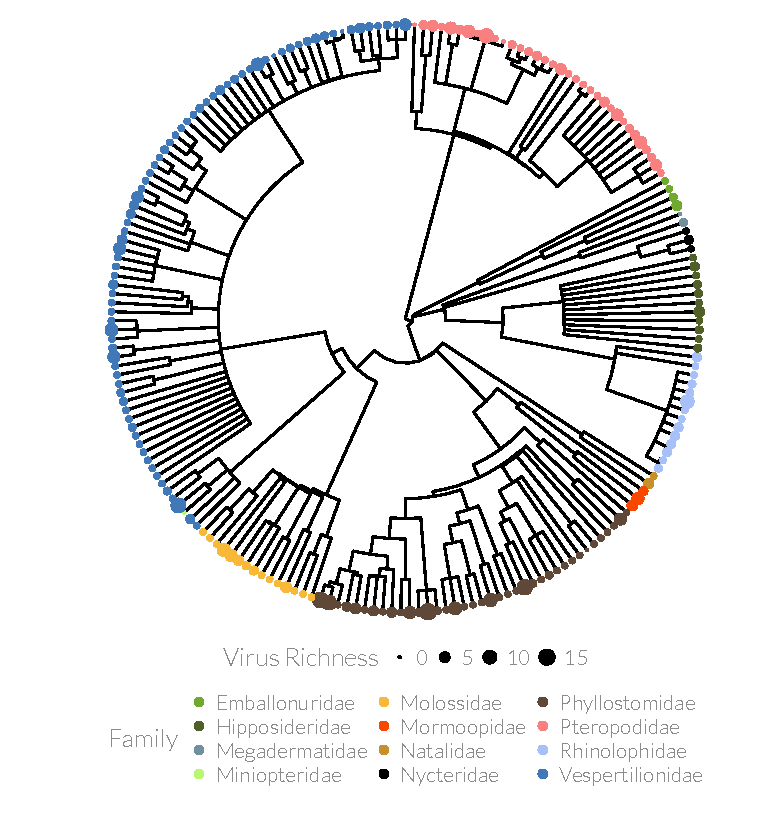
\includegraphics[width=\textwidth]{figure/treePlot-1} 

}

\caption[Pruned phylogeny with dot size showing number of pathogens and colour showing family]{Pruned phylogeny with dot size showing number of pathogens and colour showing family.}\label{fig:treePlot}
\end{figure}


\end{knitrout}










I used two measures of population structure. 
Gene flow and the number of subspecies.
The number of subspecies was counted using the Wilson and Reeder taxonomy \cite{wilson2005mammal}.
Gene flow is calculated from estimates of $F_{ST}$ collated from the literature.
Studies are from a wide range of spatial scales, from local ($\sim\SI{10}{\kilo\metre}$) to continental.
As $F_{ST}$ often increases with spatial scale \cite{burland1999population, hulva2010mechanisms, o2015genetic, vonhof2015range} I controlled for this by only using data from studies where a large proportion of the species range was studied.
I used the ratio of the furthest distance between $F_{ST}$ samples (measured with \url{http://www.distancefromto.net/} if not stated) to the width of the IUCN species range \cite{iucn} and only used studies if this ratio was greater than 0.2.
This is an arbitrary value that was a comprimise between retaining a reasonable number of data points and controlling for the bias in spatial scale.
I converted all $F_{ST}$ value to migration using $M = \frac{1-F_{ST}}{8F_{ST}}$.
This removes the $(0, 1)$ bounds of $F_{ST}$ and is more easily interpretable though the results are unaffected. 
These two measures of population structure were analysed separately as the number of subspecies has 196 data points while there is only $F_{ST}$ data for 22 bat species.
For the subspecies analysis all bat species in \textcite{luis2013comparison} were used (i.e. all species with at least one known virus species).
However, for the gene flow analysis, all bat species with suitable $F_{ST}$ estimates were used.
As this included some species not present in \textcite{luis2013comparison} this includes some bat species with zero known virus species. 

To control for study bias I collected the number of Pubmed and Google Scholar citations for each bat species name including synonyms from ITIS \cite{itis} via the taxize package \cite{chamberlain2013taxize}.
The counts were scraped using the rvest package \cite{rvest}.
I log transformed these variables as they were strongly right skewed.
The log number of citations on Pubmed and Google scholar were highly correlated (pgls: $t$ = 19.32, df = 194, $p$ = 0).
As this correlation is strong, the results here are for analyses using only Google Scholar citations.
%See the appendix for analyses run using Pubmed citations.

Measures of body mass are taken from Pantheria \cite{jones2009pantheria} and primary literature \cite{canals2005relative, arita1993rarity, lopez2014echolocation, orr2013does, lim2001bat, aldridge1987turning, ma2003dietary, owen2003home, henderson2008movements, heaney2012nyctalus, oleksy2015high, zhang2009recent}. 
\emph{Pipistrellus pygmaeus} was assigned the same mass as \emph{P. pipistrellus} as they indistinguishable by mass.
Body mass measurements were log transformed as they were strongly right skewed.
Distribution size was estimated by downloading range maps for all species from IUCN \cite{iucn} and were also logged due to right skew.


To control for phylogenetic nonindependance I used the best-supported phylogeny from \textcite{fritz2009geographical} (shown in Figure~\ref{fig:treePlot}) which is the supertree from \cite{bininda2007delayed} with names updated to match the Wilson \& Reeder taxonomy \cite{wilson2005mammal}.
Phylogenetic manipulation was performed using the ape package \cite{ape}.
The importance of the phylogeny on each variable separately (the $\lambda$ parameter of the variable regressed against an intercept) was estimated and tested against the null of $\lambda = 0$ with log-likelihood ratio tests using caper \cite{caper}.
I also performed the analysis using the tree from \cite{jones2005bats} as this has some broad changes with families in different places.
However the phylogeny did not affect the analysis.







		
		























\begin{knitrout}\footnotesize
\definecolor{shadecolor}{rgb}{0.969, 0.969, 0.969}\color{fgcolor}\begin{figure}[t]

{\centering 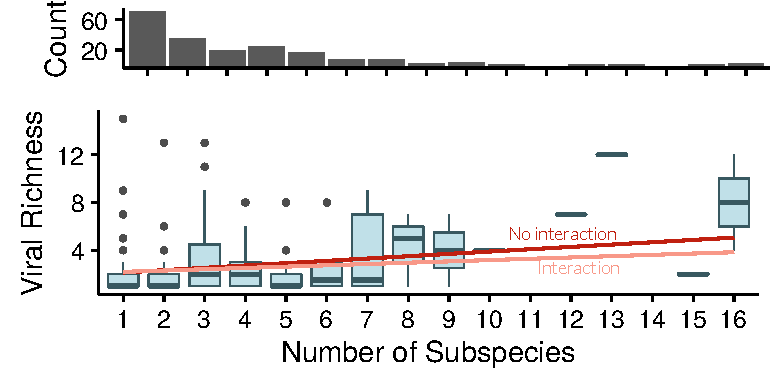
\includegraphics[width=0.8\textwidth]{figure/boxplot-1} 

}

\caption[Number of virus species against number of subspecies]{Number of virus species against number of subspecies. 		
The top panel shows the distribution of the data, with most species having few subspecies.		
Data within a number of subspecies are plotted as boxplots with the dark bar showing the median, the box showing the interquartile range, vertical lines showing the range and outliers shown as seperate points.		
Regression lines are from multivariate phylogenetic models with all other independant variables set at their median value.		
The models shown are those with (pink) and without (red) an interaction between study effort and number of subspecies.		
}\label{fig:boxplot}
\end{figure}


\end{knitrout}






%%%%%%%%%%%%%%%%%%%%%%%%%%%%%%%%%%%%%%%%%%%%%%%%%%%%%%%%%%%%%%%%%%%%%%%%%%%%%%%%%%%%%%%%%%%%%%%%%%%%%%%%%%%%%%%%%%%%%%%%%%%%%%%%%%%%%%%%%%%%%%%%%%%%%%%%%%%
%%%% FST ANALYSIS                                                                                                                                  %%%%%%%%
%%%%%%%%%%%%%%%%%%%%%%%%%%%%%%%%%%%%%%%%%%%%%%%%%%%%%%%%%%%%%%%%%%%%%%%%%%%%%%%%%%%%%%%%%%%%%%%%%%%%%%%%%%%%%%%%%%%%%%%%%%%%%%%%%%%%%%%%%%%%%%%%%%%%%%%%%%%



























































\begin{knitrout}\footnotesize
\definecolor{shadecolor}{rgb}{0.969, 0.969, 0.969}\color{fgcolor}\begin{figure}[t]

{\centering 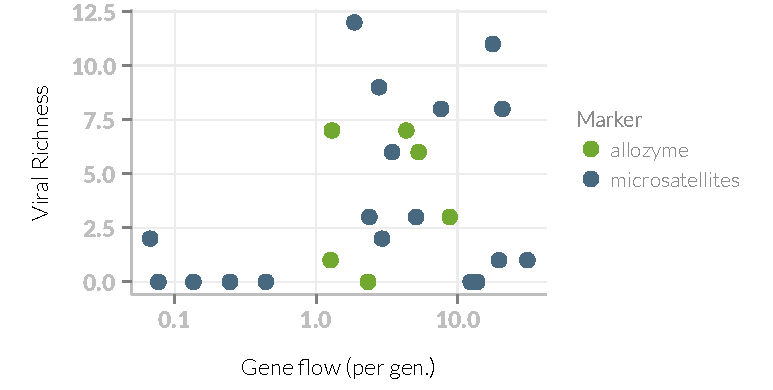
\includegraphics[width=0.8\textwidth]{figure/fstRawData-1} 

}

\caption[Gene flow per generation (on a log scale) against viral richness]{Gene flow per generation (on a log scale) against viral richness. The genetic marker used is shown with colour. The red line shows the univariate phylogenetic model.}\label{fig:fstRawData}
\end{figure}


\end{knitrout}



\begin{knitrout}\footnotesize
\definecolor{shadecolor}{rgb}{0.969, 0.969, 0.969}\color{fgcolor}\begin{figure}[t]

{\centering 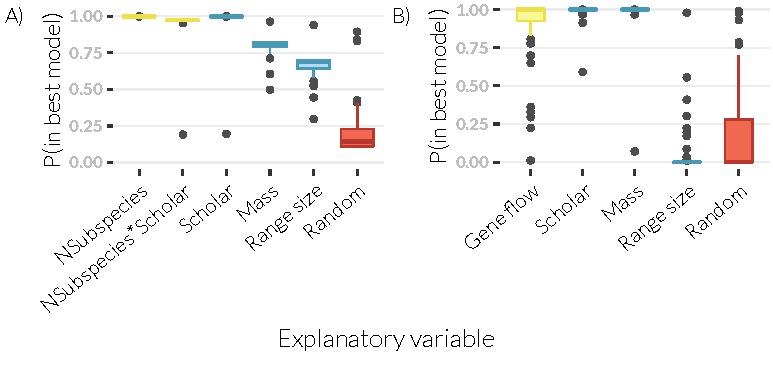
\includegraphics[width=\textwidth,trim = 0 1cm 0 0]{figure/fstITPlots-1} 

}

\caption[Akaika variable weights for $F_{ST}$ analysis.]{Akaika variable weights for both analyses. The probability that each variable will be in the best model if the data were recollected is shown for each of the bootstrap analyses. The purple ``Random'' box is a uniform random variable used as a null. Population structure (Number of subspecies and Gene flow), shown in red, is likely to be in the best model in both analyses.}\label{fig:fstITPlots}
\end{figure}


\end{knitrout}



%$F_{ST}$ studies are conducted at a range of spatial scales, but $F_{ST}$ often increases with distance studied \cite{burland1999population, hulva2010mechanisms, o2015genetic, vonhof2015range}.
%To minimise the effects of this I only used data from studies that cover rangeUseable * 100\% of the diameter of the species range.
%This is a largely arbitrary value that could be considered to reflect a ``global'' estimate of $F_{ST}$ while keeping a reasonable number of datapoints available.
%I calculated the diameter of the species range by finding the furthest apart points in the IUCN species range \cite{iucn} even if the range is split into multiple polygons.
%The width covered by each study was the distance between the most distant sampling sites.
%When this was not explicit in the paper, the centre of the lowest level of geographic area was used.



\subsection{Statistical analysis}

Statistical analysis for both dependant variables was conducted using a information theoretical/model averaging approach \cite{burnham2002model} specifically following \cite{whittingham2005habitat, whittingham2006we}.
I chose a credible set of models including all combinations of independent variables and a model with just an intercept.
In the analysis using the number of subspecies dependant variable I also included an interaction term between study effort and number of subspecies.
This interaction was included as I believed \emph{a priori} that this interaction may be present as subspecies in well studied species are more likely to be identified.
The interaction was only included in models with both study effort and number of subspecies as individual terms.

I fitted phylogenetic regressions of all models using nlme \cite{nlme}.
The independant variables were centered and scaled to allow direct comparison of the coefficients \cite{schielzeth2010simple}.
In each case I simultaneously fitted the $\lambda$ parameter as this avoids mispecifying the model \cite{revell2010phylogenetic}.
$\kappa$ and $\delta$ parameters were constrained to one as they are more concerned with when along a branch evolution occurs and because fitting multiple parameters makes interpretation difficult. 

To establish the importance of variables I calculated the probability, $Pr$, that each variable would be in the best model if the data were recollected.
For each variable the mean of it's coefficient, $\beta$, in all models that contained that variable was also calculated to determine the direction and strength of the variables.
In the subspecies analysis, this mean of $\beta$ was calculated for all models, only models with a interaction term and only models without an interaction.
As the interaction term greatly affects the estimated value of $\beta$, considering these value seperately aids interpretation.
Following \cite{whittingham2005habitat} I included a uniformally random variable as a null variable as even unimportant variables can have Akaiki weights notably greater than zero.
The whole analysis was run 50 times, resampling the random variable each time.
I calculated AICc for each model.
I calculated the average AICc, $\bar{\text{AICc}}$, by averaging AICc scores within models.
$\Delta\text{AICc}$ was calculated as $\text{min}(\bar{\text{AICc}}) - \bar{\text{AICc}}$, not the mean of the individual $\Delta\text{AICc}$ scores, to guarantee that the best model has $\Delta\text{AICc} = 0$.
From these $\Delta\text{AICc}$ I calculated Akaiki weights, $w$.
This value can be interpreted as the probability that a model would be the best model if the data were recollected.
For each variable, the sum of the Akaiki weights of models containing that variable are summed to give $Pr$.
This value can be interpreted as the probability that the given variable is in the best model.



%%%%%%%%%%%%%%%%%%%%%%%%%%%%%%%%%%%%%%%%%%%%%%%%%%%%%%%%%%%%%%%%%%%%%%%%%%%%%%%%%%%%%%%%%%%%%%%%%%%%%%%%%%%%%%%%%%%%%%%%%%%%%%%%%%%%%%%%%%%%%%%%%%%%%%%%%%%

\section{Results}

%%%%%%%%%%%%%%%%%%%%%%%%%%%%%%%%%%%%%%%%%%%%%%%%%%%%%%%%%%%%%%%%%%%%%%%%%%%%%%%%%%%%%%%%%%%%%%%%%%%%%%%%%%%%%%%%%%%%%%%%%%%%%%%%%%%%%%%%%%%%%%%%%%%%%%%%%%%

\subsection{Number of Subspecies}
\tmpsection{More descriptive}

After data cleaning there was data for 196 bat species in 11 families.
There appears to be a positive relationship between the number of subspecies and viral richness (Figure~\ref{fig:boxplot}) though few species have more than four subspecies. 
The number of described virus species for a bat host ranged up to 15 viruses in \emph{Carollia perspicillata}.
Figure~\ref{fig:treePlot} shows the phylogeny used and the number of viruses for each species.
The mean number of viruses across families is fairly constant with a lower range of 1.67 for Nycteridae.
The highest mean is Mormoopidae with 5 virus species per bat species, but this is based on a sample size of 3.
The Phyllostomidae have the second highest mean  of 3.49 (n = 37).

The small change in mean pathogen richness across families and the lack of clear pattern in Figure~\ref{fig:treePlot} implies that viral richness is not strongly phylogenetic. 
This is corroborated by the small estimated size of $\lambda$ ($\lambda$ = 0.04, $p$ = 0.21).
This fact implies that other factors must control pathogen richness.
It also implies that pathogens are not directly inherited down the phylogeny, although this is to be expected by the fast evolution of viruses.

Of the explanatory variables, the number of subspecies has no phylogenetic autocorrelation ($\lambda$ = \ensuremath{10^{-6}}, $p$ = 1), study effort and distribution size have weak but significant autocorrelation (Study Effort: $\lambda$ = 0.1, $p$ = \ensuremath{9.12\times 10^{-3}}, Distribution size: $\lambda$ = 0.46, $p$ = \ensuremath{2.82\times 10^{-9}}) and mass is strongly phylogenetic ($\lambda$ = 0.93, $p$ = 0). 
The parameter $\lambda$ is fitted and governs how important the phylogeny is in the model.
Across all models the mean value of $\lambda$ is 0.08 implying the residuals from the model are weakly phylogenetic.
A small number of models (0.4\%)  had negatively phylogenetically distributed residuals.

\tmpsection{Model results}

Summing the Akaiki weights of all models that contain a given variable gives a probability, $Pr$, that the variable would be in the best model (Figure~\ref{fig:fstITPlots}A) if the data were recollected \cite{whittingham2006we}.
The number of subspecies is very likely in the best model ($Pr > $ 0.99) as is the interaction between number of species and study effort ($Pr = $ 0.96) compared to the benchmark random variable which has $Pr = $ 0.21.
When models with the interaction term are removed, on average (mean weighted by Akaiki weights) there is a positive relationship between the number of subspecies and viral richness ($\beta = $ 0.63, variance = 0.02).
Models with an interaction between number of subspecies and study effort have a positive interaction term ($\beta = $ 0.5, variance = \ensuremath{5.11\times 10^{-5}}) and a negative linear term ($\beta = $ 0.31, variance = \ensuremath{2.13\times 10^{-4}}) which in total is a positive relationship for most of the range of the study effort data.
This supports the hypothesis that population structure promotes pathogen richness.
The strong support for a positive interaction term implies that strong population structure only predicts high known pathogen richness in the presence of high study effort.
One interpretation of this is that population structure alone does not predict high known richness; reasonable study effort is still needed to turn the expected high richness into known and recorded viral richness.
Another interpretation is that having few subspecies does not predict low viral richness unless the species has been suitable sampled; the low number of subspecies is probably due to a lack of study rather than an accurate measurement.
As seen in Figure~\ref{fig:fstITPlots}A, study effort is very likely in the best model ($\beta = $ 0.99, $Pr > $ 0.98) body mass and range size are also probably in the best model ($\beta = $ 0.48, $Pr = $ 0.8 and $\beta = $ 0.35, $Pr = $ 0.66).



\begin{table}[t]
\centering
\caption[Estimated variable weights and coefficients]{
Estimated variable weights (probability that a variable is in the best model) and their estimated coefficients for both number of subspecies and gene flow analyses.
The coefficients for number of subspecies are also seperated for models with and without the interaction term because this term strongly changes the coefficient. 
However, there are no weights for these seperated terms as they are not directly compared in the model selection framework.
}
%\rowcolors{2}{gray!25}{white}
\begin{tabular}{@{}>{\small}l rrrr@{}}
\toprule
& \multicolumn{2}{c}{\textit{Number of Subspecies}} & \multicolumn{2}{c}{\textit{Gene flow}}\\\cmidrule(rl){2-3}\cmidrule(rl){4-5}
\normalsize{Variable} & $Pr$ & Coefficient & $Pr$ & Coefficient\\
\midrule
Number of subspecies &&&&\\
\hspace{3mm}Total & 1.00 & 0.32 &&\\
\hspace{3mm}Models without interaction term &&  0.63 &&\\
\hspace{3mm}Models with interaction term &&  0.31 &&\\
Number of subspecies:log(Scholar) &  0.96 &  0.50 && \\[2.5mm]  
Gene flow & & &  0.89 &  \ensuremath{-0.67}\\[2.5mm]  
log(Scholar) &  0.98 &  0.99 & 
   0.99 &  2.49\\
log(Mass) &  0.80 &  0.48 & 
   0.98 &  \ensuremath{-0.35}\\
log(Range size) &  0.66 &  0.35& 
   0.06 &  1.57\\
Random &  0.21 &  0.05& 
   0.18 &  0.23\\
\bottomrule
\end{tabular}

\label{t:fstmodels}
\end{table}



\subsection{Gene Flow}

\tmpsection{More Descriptive}
Due to the low number of studies and the restrictive requirements imposed on study design, there are only data for 24 bat species in 7 families.
The number of described virus species for a bat host ranged up to 12 viruses in \emph{Miniopterus schreibersii}.
%Figure~\ref{fig:fstTreePlot} shows the phylogeny used and the number of viruses for each species.



\begin{table}[t]
\centering
%\rowcolors{2}{gray!25}{white}
\caption[Model selection results for number of subspecies analysis]{
Model selection results for number of subspecies and gene flow analysis. 
$\bar{\text{AICc}}$ is the mean AICc score across 50 resamplings of the null random variable. 
$\Delta$AICc is the $\bar{\text{AICc}}$ score minus the lowest score. 
$w$ is the Akaike weight and can be interpreted as the probability that the model is the best model (of those in the plausible set).
$\sum w_i$ is the cumulative sum of the Akaike weights.
log(Scholar)*NSubspecies implies the interaction term between study effort and number of subspecies as well as both of the individual linear terms.
In the number of subspecies analysis there are many models with low $\Delta$AICc scores suggesting there there is no single `best model'.
In the gene flow analysis, only the top model is supported.
}

\begin{tabular}{@{}>{\small}lrrrr@{}}

\toprule
\normalsize{Model} & $\bar{\text{AICc}}$ & $\Delta$AICc & $w$ & $\sum w$\\
\midrule
&&&&\\[-3mm]
\textit{Number of Subspecies} &&&&\\
log(Scholar)*NSubspecies + rand & 
882 & 0.00 &
0.38 & 0.38\\
log(Scholar)*NSubspecies & 
884 & 1.39 &
0.19 & 0.57\\
log(Scholar)*NSubspecies + rand + log(Mass) & 
885 & 2.24 &
0.12 & 0.70\\
log(Scholar)*NSubspecies  + log(Mass) & 
885 & 3.14 &
0.08 & 0.78\\
log(Scholar)*NSubspecies  + log(Mass) + log(RangeSize) & 
886 & 3.18 &
0.08 & 0.86\\
log(Scholar)*NSubspecies  + rand + log(RangeSize) & 
886 & 3.94 &
0.05 & 0.91\\
log(Scholar)*NSubspecies  + log(RangeSize) & 
886 & 3.95 &
0.05 & 0.96\\
log(Scholar) + NSubspecies & 
889 & 6.93 &
0.01 & 0.97\\
log(Scholar) + NSubspecies + log(Mass) & 
890 & 7.80 &
0.01 & 0.98\\[2mm]
\textit{Gene flow} &&&&\\
log(Scholar) + log(Gene flow) + log(Mass) & 
71 & 0.00 &
1.00 & 1.00\\
log(Scholar) + log(Mass) & 
105 & 34.09 &
0.00 & 1.00\\
log(Mass) + log(Range size) & 
106 & 35.06 &
0.00 & 1.00\\
%log(Scholar) + log(Gene flow) + log(Mass) + rand &
%round(fstModelWeights[4 ,2]) & sprintf("%.2f", round(fstModelWeights[4, 3], 2)) &
%sprintf("%.2f", round(fstModelWeights[4, 4], 2)) & sprintf("%.2f", round(fstModelWeights[4, 5], 2))\\
\bottomrule
\end{tabular}

\label{t:subsmodels}
\end{table}

As with the Number of Subspecies dataset, there is no phylogenetic signal in the number of virus species ($\lambda$ = \ensuremath{10^{-6}}, $p$ = 1)
Gene flow also has no phylogenetic autocorrelation ($\lambda$ = \ensuremath{10^{-6}}, $p$ = 1).
Due to the low sample size, significance tests are unlikely to have much power.
However, study effort has some phylogenetic autocorrelation ($\lambda$ = 0.15, $p$ = 0.56) while distribution size and mass seem to show phylogenetic signal (Distribution size: $\lambda$ = 0.67, $p$ = 0.53, Mass: $\lambda$ = 0.79, $p$ = \ensuremath{2.69\times 10^{-3}}).


\tmpsection{Model results}

While less strongly supported than the number of subspecies, gene flow is likely in the best model ($Pr = $ 0.89) compared to the benchmark random variable which has $Pr = $ 0.18 as shown in Figure~\ref{fig:fstITPlots}B.
On average (mean weighted by Akaiki weights) there is a negative relationship between gene flow and viral richness ($\beta = $ \ensuremath{-0.67}, variance = \ensuremath{5.48\times 10^{-3}}) despite the apparent positive relationship (see Figure~\ref{fig:fstRawData}) weakly suggested by the bivariate model (pgls: $\beta$ = 0.63, $t$ = 1.16, df = 13, $p$ = 0.27).
This supports the hypothesis that population structure promotes viral richness.
Possibly due to the smaller sample size, or a weaker relationship, this coefficient is much more varied than the number of subspecies coeficient with 21.75\% of models estimating a positive relationship.

As in the number of subspecies analysis, study effort is very likely in the best model ($Pr = $ 0.99) as is body mass ($Pr = $ 0.98).
However, body mass has a negative average coefficient ($\beta = $ \ensuremath{-0.35}, variance = 0.04) which is in contrast to number of subspecies analysis, many studies in the literature \cite{kamiya2014determines, turmelle2009correlates, gay2014parasite, maganga2014bat} and the bivariate model (pgls: $\beta$ = 0.6, $t$ = 0.38, df = 13, $p$ = 0.71).
In contrast to the number of subspecies analysis, range size is almost certainly not in the best model with $Pr = $ 0.06 being much less than the random variable.
This variable being less supported than the random variable is probably because range size is closely correlated with study effort (pgls: $\beta$ = 0.6, $t$ = 4.45, df = 13, $p$ = \ensuremath{6.58\times 10^{-4}}).

Across all models the mean value of $\lambda$ is \ensuremath{-1.64} and a large number of individual models (58.09\%)  had negatively phylogenetically distributed residuals implying the residuals from the model are strongly negatively phylogenetic.
Due to the small sample size this is probably due to a small number of data points with large residuals being distant on the tree.









%\begin{table}[t]
%\centering
%%\rowcolors{2}{gray!25}{white}
%\caption[Model selection results for number of subspecies analysis]{
%Model selection results for number of subspecies analysis. 
%$\bar{\text{AICc}}$ is the mean AICc score across nBoots resamplings of the null random variable. 
%$\Delta$AICc is the $\bar{\text{AICc}}$ score minus the lowest score. 
%$w_i$ is the Akaike weight and can be interpreted as the probability that the model is the best model (of those in the plausible set).
%$\sum w_i$ is the cumulative sum of the Akaike weights.
%}
%
%\begin{tabular}{@{}>{\small}lrrrr@{}}
%
%\toprule
%\normalsize{Model} & $\bar{\text{AICc}}$ & $\Delta$AICc & $w_i$ & $\sum w_i$\\[2em]
%\midrule
%\textit{Number of Subspecies} &&&&\\
%log(Scholar)*NSubspecies + rand & 
%round(modelWeights[1 ,2]) & sprintf("%.2f", round(modelWeights[1, 3], 2)) &
%sprintf("%.2f", round(modelWeights[1, 4], 2)) & sprintf("%.2f", round(modelWeights[1, 5], 2))\\
%log(Scholar)*NSubspecies & 
%round(modelWeights[2 ,2]) & sprintf("%.2f", round(modelWeights[2, 3], 2)) &
%sprintf("%.2f", round(modelWeights[2, 4], 2)) & sprintf("%.2f", round(modelWeights[2, 5], 2))\\
%log(Scholar)*NSubspecies + rand + log(Mass) & 
%round(modelWeights[3 ,2]) & sprintf("%.2f", round(modelWeights[3, 3], 2)) &
%sprintf("%.2f", round(modelWeights[3, 4], 2)) & sprintf("%.2f", round(modelWeights[3, 5], 2))\\
%log(Scholar)*NSubspecies  + log(Mass) & 
%round(modelWeights[4 ,2]) & sprintf("%.2f", round(modelWeights[4, 3], 2)) &
%sprintf("%.2f", round(modelWeights[4, 4], 2)) & sprintf("%.2f", round(modelWeights[4, 5], 2))\\
%log(Scholar)*NSubspecies  + log(Mass) + log(RangeSize) & 
%round(modelWeights[5 ,2]) & sprintf("%.2f", round(modelWeights[5, 3], 2)) &
%sprintf("%.2f", round(modelWeights[5, 4], 2)) & sprintf("%.2f", round(modelWeights[5, 5], 2))\\
%log(Scholar)*NSubspecies  + rand + log(RangeSize) & 
%round(modelWeights[6 ,2]) & sprintf("%.2f", round(modelWeights[6, 3], 2)) &
%sprintf("%.2f", round(modelWeights[6, 4], 2)) & sprintf("%.2f", round(modelWeights[6, 5], 2))\\
%log(Scholar)*NSubspecies  + log(RangeSize) & 
%round(modelWeights[7 ,2]) & sprintf("%.2f", round(modelWeights[7, 3], 2)) &
%sprintf("%.2f", round(modelWeights[7, 4], 2)) & sprintf("%.2f", round(modelWeights[7, 5], 2))\\
%log(Scholar) + NSubspecies & 
%round(modelWeights[8 ,2]) & sprintf("%.2f", round(modelWeights[8, 3], 2)) &
%sprintf("%.2f", round(modelWeights[8, 4], 2)) & sprintf("%.2f", round(modelWeights[8, 5], 2))\\
%log(Scholar) + NSubspecies + log(Mass) & 
%round(modelWeights[9 ,2]) & sprintf("%.2f", round(modelWeights[9, 3], 2)) &
%sprintf("%.2f", round(modelWeights[9, 4], 2)) & sprintf("%.2f", round(modelWeights[9, 5], 2))\\[2em]
%\textit{Gene Flow} &&&&
%log(Scholar) + log(Gene flow) + log(Mass) & 
%round(fstModelWeights[1 ,2]) & sprintf("%.2f", round(fstModelWeights[1, 3], 2)) &
%sprintf("%.2f", round(fstModelWeights[1, 4], 2)) & sprintf("%.2f", round(fstModelWeights[1, 5], 2))\\
%log(Scholar) + log(Mass) & 
%round(fstModelWeights[2 ,2]) & sprintf("%.2f", round(fstModelWeights[2, 3], 2)) &
%sprintf("%.2f", round(fstModelWeights[2, 4], 2)) & sprintf("%.2f", round(fstModelWeights[2, 5], 2))\\
%log(Mass) + log(Range size) & 
%round(fstModelWeights[3 ,2]) & sprintf("%.2f", round(fstModelWeights[3, 3], 2)) &
%sprintf("%.2f", round(fstModelWeights[3, 4], 2)) & sprintf("%.2f", round(fstModelWeights[3, 5], 2))\\
%log(Scholar) + log(Gene flow) + log(Mass) + rand &
%round(fstModelWeights[4 ,2]) & sprintf("%.2f", round(fstModelWeights[4, 3], 2)) &
%sprintf("%.2f", round(fstModelWeights[4, 4], 2)) & sprintf("%.2f", round(fstModelWeights[4, 5], 2))\\
%\bottomrule
%\end{tabular}



%%%%%%%%%%%%%%%%%%%%%%%%%%%%%%%%%%%%%%%%%%%%%%%%%%%%%%%%%%%%%%%%%%%%%%%%%%%%%%%%%%%%%%%%%%%%%%%%%%%%%%%%%%%%%%%%%%%%%%%%%%%%%%%%%%%%%%%%%%%%%%%%%%%%%%%%%%%

%\clearpage
\section{Discussion}  

%%%%%%%%%%%%%%%%%%%%%%%%%%%%%%%%%%%%%%%%%%%%%%%%%%%%%%%%%%%%%%%%%%%%%%%%%%%%%%%%%%%%%%%%%%%%%%%%%%%%%%%%%%%%%%%%%%%%%%%%%%%%%%%%%%%%%%%%%%%%%%%%%%%%%%%%%%%

\tmpsection{Restate results}

I have tested the hypothesis that population structure promotes pathogen richness in bats.
By analysing data on two measures of population structure, and using larger datasets than previous studies, it is hoped that any conclusions may be more robust than the conflicting results in the literature \cite{gay2014parasite, turmelle2009correlates, maganga2014bat}.
I have found that a positive affect of population structure (a positive effect of the number of subspecies and a negative effect of gene flow) are likely to be in the best models for explaining viral richness.
Study effort is also clearly supported confirming the expectation that additional study of a bat species yields more known viruses infecting that species and highlighting again that this bias cannot be ignored in studies using known pathogen richness as a proxy for total pathogen richness.


\tmpsection{Weaknesses and limitations}

Although I have used measures of study effort to try to control for biases in the viral richness data, this bias could still make the results here unreliable --- this is especially true as study effort is by far the strongest predictor of viral richness in both datasets.
It is hoped that as untargeted sequencing of viral genetic material (e.g. \textcite{anthony2013strategy}) becomes cheaper and more common this bias can be reduced.
The strength of the relationship between study effort and known viral richness also highlights the number of virus species and bat-virus host-pathogen relationships yet to be discovered.

I have used two measures of pathogen richness and the number of subspecies dataset is larger than those used in previous studies.
However it is clear that the gene flow dataset is small (n = 24).
Furthermore, while the model averaging approach has given a negative model averaged coefficient, the univariate model of gene flow against viral richness gave a positive coefficient.
It is not easy to interpret these contradictions but it is clear that the results from the gene flow analysis alone should not be considered strong evidence for a relationship between pathogen richness and population structure.
The sensitivity of this analysis reiterates the need to use large datasets where possible and use mutliple measures of population structure to promote robust conclusions.

\tmpsection{Broader context of results}

The results here suggest that there is a positive relationship between population structure and pathogen richness in bats.
This is in agreement with \cite{maganga2014bat, turmelle2009correlates} but in disagreement with \cite{gay2014parasite}.
Furthermore it contradicts the assumption that factors that promote high $R_0$ will automatically promote high pathogen richness \cite{nunn2003comparative, morand2000wormy}.

This relationship implies that direct or indirect competitive mechanisms are acting such that population structure is needed in order to allow escape from competition.
%Another potential mechanism by which structure might be promoting increased richness is by slowing the spread of highly virulent viruses such as rabies and preventing them from having short, intense epidemics followed by extinction \cite{}.
%This mechanism has interesting parallel to metapopulation theory in ecology in which a metapopulation structure can allow persistence of species that would otherwise go extinct.

The relationship between population structure and pathogen richness suggests that population structure has a least some potential as being predictive of high pathogen richness and therefore of a species likelihood of being a reservoir of a potentially zoonotic pathogen. 
However given that it is difficult to measure population structure and given that the relationship appears to be weak at best, this trait on it's own is unlikely to be useful in predicting zoonotic risk.
However, as a number of other factors are also associated with pathogen richness (body mass and to a lesser extent range size here but also other traits elsewhere), using a combination traits in a predictive (i.e. machine learning) framework has potential to be used in prioritising zoonotic disease surveillance.
The main hurdle in this approach is finding a way to validate models --- due to the study effort bias in current data, predictive models will also be biased.

The relationship between pathogen richness and population structure also has implications for habitat fragmentation and range shifts due to global change.
In short habitat fragmentation and range shifts that reduce movement between populations would be predicted to increase pathogen richness.
However, depending on the mechanisms by which population structure increase pathogen richness this may not be a cause for concern.
I the main mechanism is one that reduces pathogen extinction rates, a newly fragmented population is unlikely to increase it's pathogen richness over any appreciable timescale.
If however population structure actively promotes the evolution of new pathogen strains or allows the persistence of more virulent strains this could have important public health implications.
Therefore further study on the exact mechanisms by which population structure affects pathogen richness is needed. 

\tmpsection{Conclusions}

In conclusion, this study adds to the evidence that population structure may promote pathogen richness.
It does not support the view that factors that increase $R_0$ will increase pathogen richness.
Using larger datasets and multiple measurements makes the weight of the evidence here stronger than in previous studies.
However, caution must still be taken in interpreting these results as the data is biased and sparse and the analyses show that small changes in model and data choice can give opposite results.





%%%%%%%%%%%%%%%%%%%%%%%%%%%%%%%%%%%%%%%%%%%%%%%%%%%%%%%%%%%%%%%%%%%%
%%%% Repeat analysis with bat clocks and rocks                  %%%%
%%%%%%%%%%%%%%%%%%%%%%%%%%%%%%%%%%%%%%%%%%%%%%%%%%%%%%%%%%%%%%%%%%%%


\section{Appendix}















